%!TEX TS-program = xelatex
%!TEX encoding = UTF-8 Unicode

% Project note
% 	1. 一定要用 xelatex 進行編譯,因為有牽扯到中文字 (-shell-escape)
% 	2. 中文字體字體目前是使用Mac內建的中文字體
% 	3. Empty codeblocks will cause formatting problem
% 4. Install OxygenMono-Regular.tff
% 5. Install pygmentize

%%%%%% Page setting %%%%%%

%\documentclass[10pt,twocolumn,oneside]{article} %垂直兩欄、單面列印
%\setlength{\columnsep}{14pt} %兩欄模式的間距
%\setlength{\columnseprule}{0pt} %兩欄模式間格線粗細

\documentclass[10pt,oneside]{article}
\usepackage{pdflscape} % landscape mode
\usepackage{multicol} % two column
\usepackage{tocloft} 
\renewcommand\cftsecafterpnum{\vspace{-0.6ex}}
\renewcommand\cftsubsecafterpnum{\vspace{-0.6ex}}

\linespread{1} % 行距

\usepackage{enumitem} % Disable spacing in enumeration list
\setlist{nolistsep}

\usepackage{geometry} %定義邊界
\geometry{a4paper, total={170mm,257mm}, left=10mm, top=20mm, right=10mm}

%%%%%% Include special packages %%%%%%

%導入pdf文檔, \includepdf[pages={3,4}]{problem_statement.pdf}
\usepackage{pdfpages} 

%使用超連結, \href{http://codeforces.com/blog/entry/17974}{Codeforces}
\usepackage[colorlinks=true, urlcolor=cyan]{hyperref} 

%設定頁首頁尾
\usepackage{fancyhdr}	

% 大量註解用 , \begin{comment}  % 註解開始,  \end{comment}  % 註解結尾
\usepackage{verbatim} 

\usepackage{amsmath}
\usepackage{array}

\usepackage{graphicx}
\graphicspath{ {images/} }

%%%%%% Font setting %%%%%%

\usepackage{fontspec} %加這個就可以設定字體 

\usepackage{xeCJK} %讓中英文字體分開設置
\setmainfont{Arial}
\setCJKmainfont[BoldFont=STHeiti,ItalicFont=STKaiti]{STKaiti}  %設定中文為系統上的字型,而英文不去更動,使用原TeX字型
%\setmonofont{Courier} %等寬字體
\setmonofont{Oxygen Mono}

\XeTeXlinebreaklocale "zh" %這兩行一定要加,中文才能自動換行
\XeTeXlinebreakskip = 0pt plus 1pt 

%%%%%% lstsetting code setting %%%%%%

\usepackage{listings}
\usepackage{xcolor}

\definecolor{mygreen}{rgb}{0,0.6,0}
\definecolor{mygray}{rgb}{0.5,0.5,0.5}
\definecolor{mymauve}{rgb}{0.58,0,0.82}

\lstset{ %
	backgroundcolor=\color{black!5}, % set backgroundcolor,  choose the background color; you must add \usepackage{color} or \usepackage{xcolor}
	basicstyle=\footnotesize,   % the size of the fonts that are used for the code
	breakatwhitespace=false,   % sets if automatic breaks should only happen at whitespace
	breaklines=true,  % sets automatic line breaking
	captionpos=b,  % sets the caption-position to bottom
	frame=L, % add double line frame at the LHS of the code
	escapeinside={\%*}{*)},  % if you want to add LaTeX within your code
	keepspaces=true,  % keeps spaces in text, useful for keeping indentation of code (possibly needs columns=flexible)
	columns=flexible,
	commentstyle=\color{mygreen}, % comment style
	keywordstyle=\color{blue},  % keyword style
	%otherkeywords={*,...}, % if you want to add more keywords to the set  
	numbers=left, % where to put the line-numbers; possible values are (none, left, right)
	numbersep=7pt, % how far the line-numbers are from the code
	numberstyle=\tiny\color{mygray}, % the style that is used for the line-numbers
	stepnumber=1,  % the step between two line-numbers. If it's 1, each line will be numbered
	rulecolor=\color{black}, % if not set, the frame-color may be changed on line-breaks within not-black text (e.g. comments (green here))
	showspaces=false, % show spaces everywhere adding particular underscores; it overrides 'showstringspaces'
	showstringspaces=false, % underline spaces within strings only
	showtabs=false, % show tabs within strings adding particular underscores
	stringstyle=\color{mymauve},     % string literal style
	tabsize=4, % sets default tabsize to 4 spaces
	basicstyle=\footnotesize\ttfamily, %等寬字體 字體大小
	xleftmargin=\parindent,
	%title=\lstname % show the filename of files included with \lstinputlisting; also try caption instead of title
}

\lstdefinestyle{customc}{
	belowcaptionskip=1\baselineskip,
	breaklines=true,
	language=C++,
	showstringspaces=false,
	keywordstyle=\bfseries\color{green!40!black},
	commentstyle=\itshape\color{purple!40!black},
	identifierstyle=\color{blue},
	stringstyle=\color{orange},
}

\lstset{style=customc}

% sudo easy_install Pygments
% Add -shell-escape to compile flag
\usepackage{minted}

% Run in terminal for checking available styles: pygmentize -L styles
\usemintedstyle{friendly}
\definecolor{bg}{rgb}{0.95,0.95,0.95}
\newmintedfile[cppCode]{cpp}{ % [alias][code type]
	%bgcolor=bg,
	fontfamily=tt,
	linenos=true,
	numberblanklines=true,
	numbersep=12pt,
	numbersep=5pt,
	gobble=0,
	frame=leftline,
	framerule=0.4pt,
	framesep=2mm,
	funcnamehighlighting=true,
	tabsize=4,
	obeytabs=false,
	mathescape=false
	samepage=false, %with this setting you can force the list to appear on the same page
	showspaces=false,
	showtabs =false,
	texcl=false,
	fontsize=\footnotesize,
	breaklines=true,
}


%%%%%% 文件正式開始 %%%%%%

\begin{document} 

\begin{landscape} % landscape mode
\begin{multicols}{2} % two columns

%%%%%%%%%%%%%%%%%頁首%%%%%%%%%%%%%%%%%%%%

% for all other pages
\pagestyle{fancy}
% generate header
\fancyhead[L]{National Chung Cheng University -- CCU\_ToInfinityAndBeyond}
\fancyhead[R]{\thepage}
% \rhead{
\includegraphics[width=1cm]{buzz}}
% generate footer
%\fancyfoot[L]{\includegraphics[width=20pt]{pic.jpg}} %team profile picture
\fancyfoot[C]{for 2017 NCPC (Built on: \today)}
\fancyfoot[R]{\thepage}

% for page 1
\fancypagestyle{plain}
{
% generate header
\fancyhead[L]{National Chung Cheng University -- CCU\_ToInfinityAndBeyond}
\fancyhead[R]{\thepage}
% generate footer
%\fancyfoot[L]{\includegraphics[width=20pt]{pic.jpg}} %team profile picture
\fancyfoot[C]{for 2017 NCPC (Built on: \today)}
\fancyfoot[R]{\thepage}
}

% generate table of content on in a new page
\scriptsize
\tableofcontents
\pagestyle{fancy}

%\newpage
% \vfill
%\columnbreak

%%%%%%%%%%%%%%%%%正文%%%%%%%%%%%%%%%%%%%

%%%%%%%%%%%%%%%%機器設定%%%%%%%%%%%%%%%%%%

\begin{center}

\includegraphics[width=10cm]{buzz1}
\end{center}

\newpage
\section{Contest Setup}

\subsection{vimrc}
\lstinputlisting[style=,basicstyle=\footnotesize\ttfamily]{contest_setup/vimrc}

% \subsection{bashrc}
% \lstinputlisting[style=,language=bash,basicstyle=\footnotesize\ttfamily]{contest_setup/bashrc}

% \subsection{Grep Error and Warnings}

% \begin{lstlisting}
% g++ main.cpp 2>&1 | grep -E 'warning|error'
% \end{lstlisting}

% \subsection{C++ template}
% \cppCode{contest_setup/main.cpp}

\subsection{Java template}
%\lstinputlisting{contest_setup/Main.java}
\inputminted{java}{contest_setup/Main.java}

\subsubsection{Java Issues}
{\normalsize
\begin{enumerate}
\item Random Shuffle before sorting:\\ \mintinline{java}{Random rnd = new Random(); rnd.nextInt();}
\item Use \mintinline{java}{StringBuilder} for large output
%\item Java has strict parsing rules. e.g. using \mintinline{java}{sc.nextInt()} to read a long will result in RE
\item For class sorting, use code \mintinline{java}{implements Comparable<Class name>}. Or, use code \mintinline{java}{new Comparator<Interval>() {}} at \mintinline{java}{Collections.sort()} second argument
\end{enumerate}
}

\section{System Testing}

{\normalsize
\begin{enumerate}
% \item Setup Codeblock warning level and std=c++11
\item Test g++ (\mintinline{c++}{-Wall -Wextra -Wshadow -std=c++11}) and Java 8 compiler
\item Test if c++ and Java templates work properly on local and judge machine (\mintinline{c++}{bits/stdc++.h, auto})
\item Test "divide by 0" $\rightarrow$ RE/TLE?
\item Make a complete graph and run Floyd warshall, to test time complexity of the judge machine
% \item Make a linear graph and use DFS to test stack size
% \item Test output with extra newline and spaces
%\item Go to $Eclipse \rightarrow preference \rightarrow Java \rightarrow Editor \rightarrow Content Assist$, add $.abcdefghijklmnopqrstuvwxyz$ to auto activation triggers for Java in Eclipse
\end{enumerate}
}

%%%%%%%%%%%%%%%%%忠告%%%%%%%%%%%%%%%%%%%%

\section{Reminder}

% 
\includegraphics{sorting3}

{\normalsize
\begin{enumerate}
\item 請不要排擠隊友!要記得心平氣和的小聲討論喔!通常隊友的建議都會突破你盲點。
\item 每一題都要小心讀,尤其是IO的格式和限制都要看清楚。%Read the problem statements carefully. Input and output specifications and constraints are crucial!
\item 小心估計\textbf{時間複雜度} 和 \textbf{空間複雜度}%Estimate the \textbf{time complexity} and \textbf{memory complexity} carefully.
\item Coding 要兩人一組,要相信你隊友的實力!
\item 1WA 罰 20 分鐘! \textbf{放輕鬆,不要急},多產幾組測資後再丟。%Time penalty is 20 minutes per WA, \textbf{don't rush}!
\item 範測一定要過!產個幾組極端測資,例如 input 下限、特殊 cases 0, 1, -1、空集合等等 %Sample test cases must all be tested and passed before every submission! Test the corner cases, such as 0, 1, -1. Test all edge cases of the input specification.
\item 比賽是連續測資,一定要全部讀完再開始 solve 喔!%For continuous input problems, be sure to read in all input BEFORE terminating and start processing next the input.
\item Bus error: 有\mintinline{c++}{scanf, fgets} 但是卻沒東西可以讀取了!可能有early termination但是時機不對。 % Bus error: the code has $scanf, fgets$ but have nothing to read! Check if you have early termination but didn't handle it properly.
\item 圖論一定要記得檢查連通性。最簡單的做法就是loop過所有的點%Check connectivity of the graph if the problem statement doesn't say anything (just loop over all nodes!)
\item \mintinline{c++}{long long = int * int} 會完蛋%$long\ long = int * int$ won't work!
\item \mintinline{c++}{long long int} 的位元運算要記得用 \mintinline{c++}{1LL << 35} %Shifting for $long long int$ should be something like $1LL << 35$
%\item Don't use anonymous struct
\item 記得清理Global variable (煒杰要記得清圖喔!)
\item 建圖時要注意有無重邊!
\item c++ priority queue 是 max heap,Java 是 Min heap
\item 注意要不要建立反向圖 % UVa1112
\end{enumerate}
}

\section{Topic list}

{\normalsize
\begin{enumerate}
\item 列舉、窮舉 enumeration
\item 貪心 greedy 
\item 排序 sorting, topological sort
\item 二分搜 binary search (數學算式移項合併後查詢)
\item 爬行法 (右跑左追)Two Pointer
\item 離散化
\item Dynamic programming, 矩陣快速冪
\item 鴿籠原理 Pigeonhole 
\item 最近共同祖先 LCA (倍增法, LCA轉RMQ)
\item 折半完全列舉 (能用vector就用vector)
\item 離線查詢 Offline (DFS, LCA)
\item 圖的連通性 Directed graph connectivity -> DFS. Undirected graph -> Union Find
\item 因式分解
\item 從答案推回來
\item 寫出數學式,有時就馬上出現答案了! % CF Div2 R372 C
\item 奇偶性質
\item 串接、反轉、兩倍長度
\end{enumerate}
}

%%%%%%%%%%%%%%%%實用代碼%%%%%%%%%%%%%%%%%%

\section{Useful code}

\subsection{Leap year $O(1)$}

\mintinline{c++}{(year % 400 == 0 || (year % 4 == 0 && year % 100 != 0))}

\subsection{Fast Exponentiation $O(log(exp))$}

{\normalsize Fermat's little theorem: 若 $p$ 是質數,則$a^{p-1} \equiv 1 \pmod p$}

\cppCode{useful_code/fast_pow.cpp}

\subsection{Mod Inverse $ O(log n) $}

{\normalsize 
Case 1: $gcd(a, m) = 1$:  ax + my = gcd(a, m) = 1 (use ext$\_$gcd) \\

\noindent Case 2: $p\ is\ prime$: $a^{p - 2} \equiv a^{-1} mod\ p$ 
}

\subsection{GCD $O(log( min(a + b) ))$}

{\large 注意負數的case! C++ 是看被除數決定正負號的。}

\begin{minted}{c++}
ll gcd(ll a, ll b)
{
    return b == 0 ? a : gcd(b, a % b);
}
\end{minted}

\subsection{Extended Euclidean Algorithm GCD $O(log( min(a + b) ))$}

{\normalsize 
Bezout identity $ax + by = gcd(a, b)$, where $\mid x \mid \leq \frac b d$ and $\mid y \mid \leq \frac a d$.
}

\cppCode{useful_code/ext_gcd.cpp}

\subsection{Prime Generator $ O(n loglogn) $}
\cppCode{useful_code/prime_gen.cpp}

\subsection{C++ Reference}

\cppCode{useful_code/cppReference2.cpp}

%\subsubsection{scanf/printf reference}

%\subsubsection{Map}
%\cppCode{useful_code/map_API.cpp}

%\subsubsection{Set}
%\cppCode{useful_code/set_API.cpp}

%\subsubsection{Algorithm}
%\cppCode{useful_code/algorithm_API.cpp}

%\subsubsection{String}

%%%%%%%%%%%%%%%%%搜尋%%%%%%%%%%%%%%%%%%%%

\section{Search}

\subsection{Ternary Search $O(nlogn)$}

\begin{minted}{c++}
double l = ..., r = ....; // input
for(int i  = 0; i < 100; i++) {
    double m1 = l + (r - l) / 3, m2 = r - (r - l) / 3;
    if (f (m1) < f (m2)) // f - convex function
        l = m1;
    else
        r = m2;
}
f(r) - maximum of function
\end{minted}

% \subsection{N Puzzle}
% \cppCode{Search/n-puzzle.cpp}


%%%%%%%%%%%%%%%%資料結構%%%%%%%%%%%%%%%%%%

\section{Basic data structure}

\subsection{1D BIT}

\cppCode{DS/1D_BIT.cpp}

\subsection{2D BIT}

\cppCode{DS/2D_BIT.cpp}

\subsection{Union Find}

\cppCode{DS/unionFind.cpp}

\subsection{Segment Tree}
\cppCode{DS/segmentTree2.cpp}

\subsection{Sparse Table}
\cppCode{DS/sparse_table.cpp}

%%%%%%%%%%%%%%%%%%樹%%%%%%%%%%%%%%%%%%%%

\section{Tree}

\subsection{LCA}
\cppCode{Tree/lca.cpp}

\subsection{Tree Center}
\cppCode{Tree/TreeCenter.cpp}

\subsection{Treap}
\cppCode{Tree/treap.cpp}

%%%%%%%%%%%%%%%%%圖論%%%%%%%%%%%%%%%%%%%

\section{Graph}

\subsection{Articulation point / Bridge}
\cppCode{graph/ArticulationPointAndBridge-1.cpp}

\subsection{2-SAT}

{\normalsize 
\begin{align*}
&p \lor (q \land r)  \\
&= ((p \land q) \lor (p \land r)) \\
&p \oplus q   \\
&= \lnot ( (p \land q) \lor (\lnot p \land \lnot q))     \\
&= (\lnot p \lor \lnot q) \land (p \lor q)    
\end{align*}
}

\begin{minted}{c++}
// 建圖
// (x1 or x2) and ... and (xi or xj)
// (xi or xj) 建邊
// ~xi -> xj
// ~xj -> xi

tarjan(); // scc 建立的順序是倒序的拓璞排序
for (int i = 0; i < 2 * N; i += 2) {
    if (belong[i] == belong[i ^ 1]) {
        // 無解
    }
}
for (int i = 0; i < 2 * N; i += 2) { // 迭代所有變數
    if (belong[i] < belong[i ^ 1]) { // i 的拓璞排序比 ~i 的拓璞排序大
        // i = T
    }
    else {
        // i = F
    }
}
\end{minted}

\subsection{BCC}

{\normalsize
一張無向圖上,不會產生關節點 (articulation point) 的連通分量,稱作「雙連通分量」(Biconnected Component)。\\
一張無向圖上,不會產生橋 (bridge) 的連通分量,稱作「橋連通分量」(Bridge-connected Component)。
}

\subsubsection{Biconnected Component }
{\normalsize 
    %http://www.geeksforgeeks.org/biconnected-components/
    以 Edge 做分界的話,stack 要裝入 (u - v), 並 pop 終止條件為 != (u - v) \\
    以 Articulation point 做為分界 (code below),注意有無坑人的重邊 \\
    
    用SCC的code的話,只要多判一個 u 是否為 p, 如果是的話就直接 return (加在第21行之後)
}

\subsubsection{Bridge-connected Component}
\cppCode{graph/BCC-1.cpp}

\subsection{SCC}

{\normalsize 
First of all we run DFS on the graph and sort the vertices in decreasing of their finishing time (we can use a stack).\\
Then, we start from the vertex with the greatest finishing time, and for each vertex v that is not yet in any SCC, do : for each u that v is reachable by u and u is not yet in any SCC, put it in the SCC of vertex v. The code is quite simple.
}

\cppCode{graph/SCC_AMO.cpp}

\subsection{Shortest Path}

{\normalsize 
Time complexity notations: V = vertex, E = edge \\
Minimax: $dp[u][v] = min(dp[u][v], max(dp[u][k], dp[k][v]))$ \\
}
%\subsubsection{Dijkatra}

%密集圖別用priority queue!\\
%http://amoshyc.github.io/ojsolution-build/template/graph/spfa.html
%\cppCode{graph/dijkatra.cpp}

\subsubsection{Dijkatra (next-to-shortest path) $O(VlogE)$}
{\normalsize 密集圖別用priority queue! }
% https://gist.github.com/amoshyc/f011abc6fad9b413c24b
\cppCode{graph/nextToShortestPath.cpp}

\subsubsection{SPFA}
\cppCode{graph/SPFA.cpp}
% \cppCode{graph/SPFA-1.cpp}

\subsubsection{Bellman-Ford $O(VE)$}
% UVa 558, 10449
\cppCode{graph/bellmanFord1.cpp}

\subsubsection{Floyd-Warshall $O(V^3)$}
{\normalsize 
The graph is stored using adjacency matrix. The initial state is $diagnal = 0$ and $others = INF$. (If $INF$ is int, use long long for the matrix)\\
If diagonal numbers are negative $\leftarrow$ cycle . \\
}

%UVA821 
\begin{minted}{c++}
for(int k = 0; k < N; k++)
    for(int i = 0; i < N; i++)
        for(int j = 0; j < N; j++)
            dp[i][j] = min(dp[i][j], dp[i][k] + dp[k][j]);
\end{minted}

\subsection{MST}

\subsubsection{Kruskal}

{\normalsize 
\begin{enumerate}
	\item Store the graph by $(weight, (from , to))$
	\item Sort the graph by $weight$ 
	\item Start from the smallest weight, and keep adding edges that won't form a cycle with the current MST set
	\item Early termination condition: $n - 1$ edges has been added, NOT size of the union-find set
\end{enumerate}
}

\subsubsection{Second MST}
% https://amoshyc.github.io/blog/template-ci-xiao-sheng-cheng-shu.html
\cppCode{graph/second_MST.cpp}

\subsubsection{Prim}
\cppCode{graph/prim-1.cpp}

\section{Flow}

\subsection{Max Flow (Dinic)}
%http://amoshyc.github.io/ojsolution-build/template/graph/max_flow.html
\cppCode{flow/dinic.cpp}

\subsection{Min Cost Flow}
%http://amoshyc.github.io/ojsolution-build/template/graph/min_cost_flow.html
\cppCode{flow/minCostFlow.cpp}

\subsection{Bipartite Matching, Unweighted}
%http://amoshyc.github.io/ojsolution-build/template/graph/bipartite_matching.html

{\normalsize
最大匹配數:最大匹配的匹配邊的數目\\
最小點覆蓋數:選取最少的點,使任意一條邊至少有一個端點被選擇\\
最大獨立數:選取最多的點,使任意所選兩點均不相連\\
最小路徑覆蓋數:對於一個 DAG(有向無環圖),選取最少條路徑,使得每個頂點屬於且僅屬於一條路徑。路徑長可以為 0(即單個點)\\
定理1:最大匹配數 = 最小點覆蓋數(這是 Konig 定理)\\
定理2:最大匹配數 = 最大獨立數\\
定理3:最小路徑覆蓋數 = 頂點數 - 最大匹配數\\
}

\cppCode{flow/bipartiteMatching.cpp}

%%%%%%%%%%%%%%%%%字串%%%%%%%%%%%%%%%%%%%

\section{String}

\subsection{Rolling Hash}

{\normalsize 
\begin{enumerate}
	\item Use two rolling hashes if needed.  
	\item The prime for pre-calculation can be $137$ and $257$, for modulo can be $1e9 + 7$ and $0xdefaced$ 
\end{enumerate}
}

\cppCode{string/RollingHash.cpp}

\subsection{KMP}

\cppCode{string/KMP.cpp}

\subsection{Z Algorithm}

\cppCode{string/Z_Algorithm.cpp}

\subsection{Trie}
{\normalsize 
% http://amoshyc.github.io/ojsolution-build/template/ds/trie.html
注意count的擺放位置,視題意可以擺在迴圈外
\cppCode{string/TrieAmoshyc.cpp}
}

\subsection{Suffix Array}
\cppCode{string/sa.cpp}

\section{Matrix}

\subsection{Gauss Jordan Elimination}
\cppCode{Matrix/gauss_jordan.cpp}

\subsection{Determinant}

{\normalsize 
整數版本
}

\cppCode{Matrix/matrix_det.cpp}

%%%%%%%%%%%%%%%%%幾何%%%%%%%%%%%%%%%%%%%

\section{Geometry}

{\normalsize 
\begin{enumerate}
	\item Keep things in integers as much as possible!
	\item Try not to divide
	\item If you have decimals, if they are fixed precision, you can usually just multiply all the input and use integers instead
\end{enumerate}
}

\subsection{EPS}

{\normalsize 
%$a > b \rightarrow a - b > 0 \rightarrow a - b > EPS$ (stands for positive)\\
%$a \geq b \rightarrow  a - b \geq 0 \rightarrow a - b > -EPS$ (stands for positive or zero)\\

$=0$: $fabs \leq eps$\\
$<0$: $ < -eps$\\
$>0$: $ > +eps$
}

%\subsection{Template}
% \cppCode{geometry/geometry_stanford.cpp}
\cppCode{geometry/my_geometry2.cpp}

\subsection{Rectangle area}
% https://amoshyc.github.io/blog/template-ju-xing-mian-ji-he.html
\cppCode{geometry/rect_area.cpp}

\section{Math}

\subsection{Euclid's formula (Pythagorean Triples)}

{\normalsize 
$a = p^2 - q^2 $\\
$b = 2pq \; \textbf{(always even)}$ \\
$c = p^2 + q^2$\\
}

\subsection{Difference between two consecutive numbers' square is odd}

{\normalsize 
$(k + 1)^2 - k^2 = 2k + 1$
}

\subsection{Summation}

{\normalsize 
$\sum_{k=1}^{n} 1= n$\\
$\sum_{k=1}^{n} k= \frac{n(n+1)}{2}$\\
$\sum_{k=1}^{n} k^2= \frac{n(n+1)(2n+1)}{6}$\\
$\sum_{k=1}^{n} k^3= \frac{n^2(n+1)^2}{4}$\\
}

\subsection{FFT}
%http://amoshyc.github.io/ojsolution-build/template/math/fft.html
\cppCode{Math/fft.cpp}

\subsection{Combination}

% Pi-You Uva 10943
\subsubsection{Pascal triangle}

\cppCode{Math/pascal.cpp}

\subsubsection{Lucus}

\begin{equation}
\begin{split}&\binom{n}{m} \equiv \prod_{i=0}^k \binom{n_i}{m_i} \pmod p \\
\text{where}& \\
&n = n_kp^k+n_{k-1}p^{k-1}+\cdots +n_1p+n_0, \\
&m = m_kp^k+m_{k-1}p^{k-1}+\cdots +m_1p+m_0 \\
&p \text{ is prime}
\end{split}
\end{equation}

\cppCode{Math/lucas.cpp}

\subsubsection{線性}

\cppCode{Math/combination_linear.cpp}

\subsection{Chinese remainder theorem}
%http://amoshyc.github.io/ojsolution-build/template/math/crt.html

\begin{equation}
\begin{split}
\begin{cases}
        x \equiv r_1 \pmod {m_1} \\
        x \equiv r_2 \pmod {m_2} \\
        \dots \\
        x \equiv r_n \pmod {m_n}
\end{cases}
\end{split}
\end{equation}

\cppCode{Math/chineseRemainderTheorem.cpp}

\subsection{2-Circle relations}

{\normalsize 
$d$ = 圓心距, $R$, $r$ 為半徑 ($R \geq r$)\\
內切: $d = R - r$\\
外切: $d = R + r$\\
內離: $d < R - r$\\
外離: $d > R + r$\\
相交: $d < R + r$ 且 $d > R - r$
}

\subsection{Fun Facts}

{\normalsize 
\begin{enumerate}
	\item 如果 $\frac b a$ 是最簡分數,則 $1 - \frac b a$也是%http://amoshyc.github.io/ojsolution-build/cf/cf369/pe.html
\end{enumerate}
}

\subsection{偏序集與 Dilworth}

\subsubsection{原理}
{\normalsize
Dilworth 與其對偶定理適用於嚴格偏序,也適用於非嚴格偏序。(Hasse Diagram)

\begin{enumerate}
	\item Dilworth:最小正鏈覆蓋 = 最長反鏈長度
	\item 對偶定理:最小反鏈覆蓋 = 最長正鏈長度
\end{enumerate}
}

\subsubsection{題目}

{\normalsize
R x C 的格子中 N 個點 (r[i], c[i])。\\
定義一次旅行為從任一個點出發,只能 \textbf{往右走或往下走}。\\
請問:\\
1. 經過最多點的那次旅行是經過了多少個點?\\
2. 最少須要旅行幾次才能走完所有點? \\

\noindent 即非嚴格偏序集 $P = (S, \le)$

\begin{equation}
\begin{split}
\begin{cases}
    	S &= \{ (r_i, c_i) | 0 \le i < N \} \\
    	\le &= (r_i \le r_j \land c_i \le c_j)
\end{cases}
\end{split}
\end{equation}

\noindent 題目所求分別為\\
1. 最長正鏈長度,即為最小反鏈覆蓋。\\
2. 最小正鏈覆蓋,即為最長反鏈長度。
}

\subsubsection{只能往右走或往下走}

{\normalsize
\textbf{最長正鏈長度}

\begin{enumerate}
	\item 將點排序,r 由小到大,相同時 c \textbf{由小到大}
	\item 在 c 上求最長 \textbf{單調遞增} 子序列,長度即為所求
\end{enumerate}
}

{\normalsize
\noindent \textbf{最長反鏈長度}

\begin{enumerate}
	\item 將點排序,r 由小到大,相同時 c \textbf{由小到大}
	\item 在 c 上求最長 \textbf{嚴格遞減} 子序列,長度即為所求
\end{enumerate}
}

\columnbreak
\subsubsection{只能往斜右下走}
{\normalsize
如果題目改成 \textbf{只能往斜右下走,不能向右或向下},則演算法改成
}

{\normalsize
\noindent  \textbf{最長正鏈長度}

\begin{enumerate}
	\item 將點排序,r 由小到大,相同時 c \textbf{由大到小}
	\item 在 c 上求最長 \textbf{嚴格遞增} 子序列,長度即為所求
\end{enumerate}
}

{\normalsize
\noindent \textbf{最長反鏈長度}

\begin{enumerate}
	\item 將點排序,r 由小到大,相同時 c \textbf{由大到小}
	\item 在 c 上求最長 \textbf{單調遞減} 子序列,長度即為所求
\end{enumerate}

\noindent \textbf{c 由小到大是為了防止誤判}
}

\subsubsection{最長 嚴格遞增 子序列、最長 嚴格遞減 子序列}

\cppCode{DP/dilworth_strict_inc.cpp}

\subsubsection{最長 單調遞增 子序列、最長 單調遞減 子序列:}

\cppCode{DP/dilworth_monotone_inc.cpp}

\columnbreak
\subsection{排列組合}

\subsubsection{排列 P}

{\normalsize 
$P^n_k = \frac{n!}{(n-k)!}$

\begin{enumerate}
	\item 從 $n$ 個不同球中取 $k$ 個,\textbf{不同取出順序視為不同},方法數為 $P^n_k$
	\item $P^4_2 = 12$
\end{enumerate}
}

\subsubsection{圓排列 Q}

{\normalsize
$Q^n_k = \frac{n!}{k (n-k)!} = \frac{P^n_k}{k}$

\begin{enumerate}
	\item 從 $n$ 個不同球中取 $k$ 個,\textbf{排成一個圓},圓只考慮相對位置,方法數為 $Q^n_k$
	\item $Q^4_2 = 6$
\end{enumerate}
}

\subsubsection{組合 C}

{\normalsize
\begin{equation}
\begin{split}
\begin{cases}
	C^n_n &= C^n_0 = 1 \\
	C^n_k &= C^n_{n-k} = \frac{n!}{(n-k)!k!} = \frac{P^n_k}{k!} \\
	C^n_k &= C^{n-1}_{k-1} + C^{n-1}_{k}
\end{cases}
\end{split}
\end{equation}

\begin{enumerate}
	\item 從 $n$ 個不同球中取 $k$ 個, \textbf{取出順序不影響} ,方法數為 $C^n_k$
	\item 考慮第 $k$ 顆球取或不取:取的話轉移成從 $n-1$ 個不同球中取出 $k-1$ 個;不取的話,轉移成從 $n-1$ 個球中取 $k$ 個,即 $C^n_k = C^{n-1}_{k-1} + C^{n-1}_{k}$
	\item $C^4_2 = 6$
\end{enumerate}
}

\subsubsection{重複組合 H}
{\normalsize
$H^n_k = C^{n+k-1}_k = C^{n+k-1}_{n-1}$

\begin{enumerate}
	\item 將 $n$ 顆\textbf{相同的球} 丟進 $k$ 個\textbf{可空、不同} 箱子,方法數為 $H^n_k$
	\item $x_1 + x_2 + \dots + x_n = k$,$(x_1, x_2, \dots, x_n)$ 非負整數解的個數為 $H^n_k$
	\item $x_1 + x_2 + \dots + x_n = k$,$(x_1, x_2, \dots, x_n)$ 正整數解的個數為 $H^n_{k - n}$
	\item $H^4_2 = 10$
\end{enumerate}
}

\subsubsection{Stirling Number(Type I)}
{\normalsize
\begin{equation}
\begin{split}
\begin{cases}
	S^n_0 &=0 \\
    	S^n_1 &=1 \\
    	S^n_k &= S^{n-1}_{k-1} + (n-1) S^{n-1}_{k}
\end{cases}
\end{split}
\end{equation}

\begin{enumerate}
	\item 將 $n$ 顆\textbf{不同的球} 丟進 $k$ 個 \textbf{非空、相同} 箱子,每個箱子為一 \textbf{圓排列} ,方法數為 $S^n_k$
	\item 考慮第 $n$ 顆球:可以自己一個箱子,即其他 $n-1$ 個球丟進 $k-1$ 個箱子;也可以 $n-1$ 個球丟進 $k$ 個箱子,這顆球插到任一顆球旁邊。所以得 $S^n_k = S^{n-1}_{k-1} + (n-1) S^{n-1}_{k}$
	\item $S^4_2 = 11$
\end{enumerate}
}

\subsubsection{Stirling Number(Type II)}
{\normalsize
\begin{equation}
\begin{split}
\begin{cases}
	S^n_n &= S^n_1 = 1 \\
    	S^n_k &= S^{n-1}_{k-1} + k S^{n-1}_{k}
\end{cases}
\end{split}
\end{equation}

\begin{enumerate}
	\item 將 $n$ 顆 \textbf{不同的球} 丟進 $k$ 個 \textbf{非空、相同} 箱子,每一個箱子為一 \textbf{集合},方法數為 $S^n_k$
	\item 考慮第 $n$ 顆球:可以自己一個箱子,即其他 $n-1$ 個球丟進 $k-1$ 個箱子;也可以 $n-1$ 個球丟進 $k$ 個箱子,這顆球丟進其中一個箱子。所以得 $S^n_k = S^{n-1}_{k-1} + k S^{n-1}_{k}$
	\item $S^4_2 = 7$
\end{enumerate}
}

%%%%%%%%%%%%DP%%%%%%%%%%

\section{Dynamic Programming - Problems collection}
%\cppCode{DP/dp.cpp}
\VerbatimInput{DP/dp_noComment.txt}

\columnbreak
\cppCode{DP/TSP.cpp}

%trig information
% 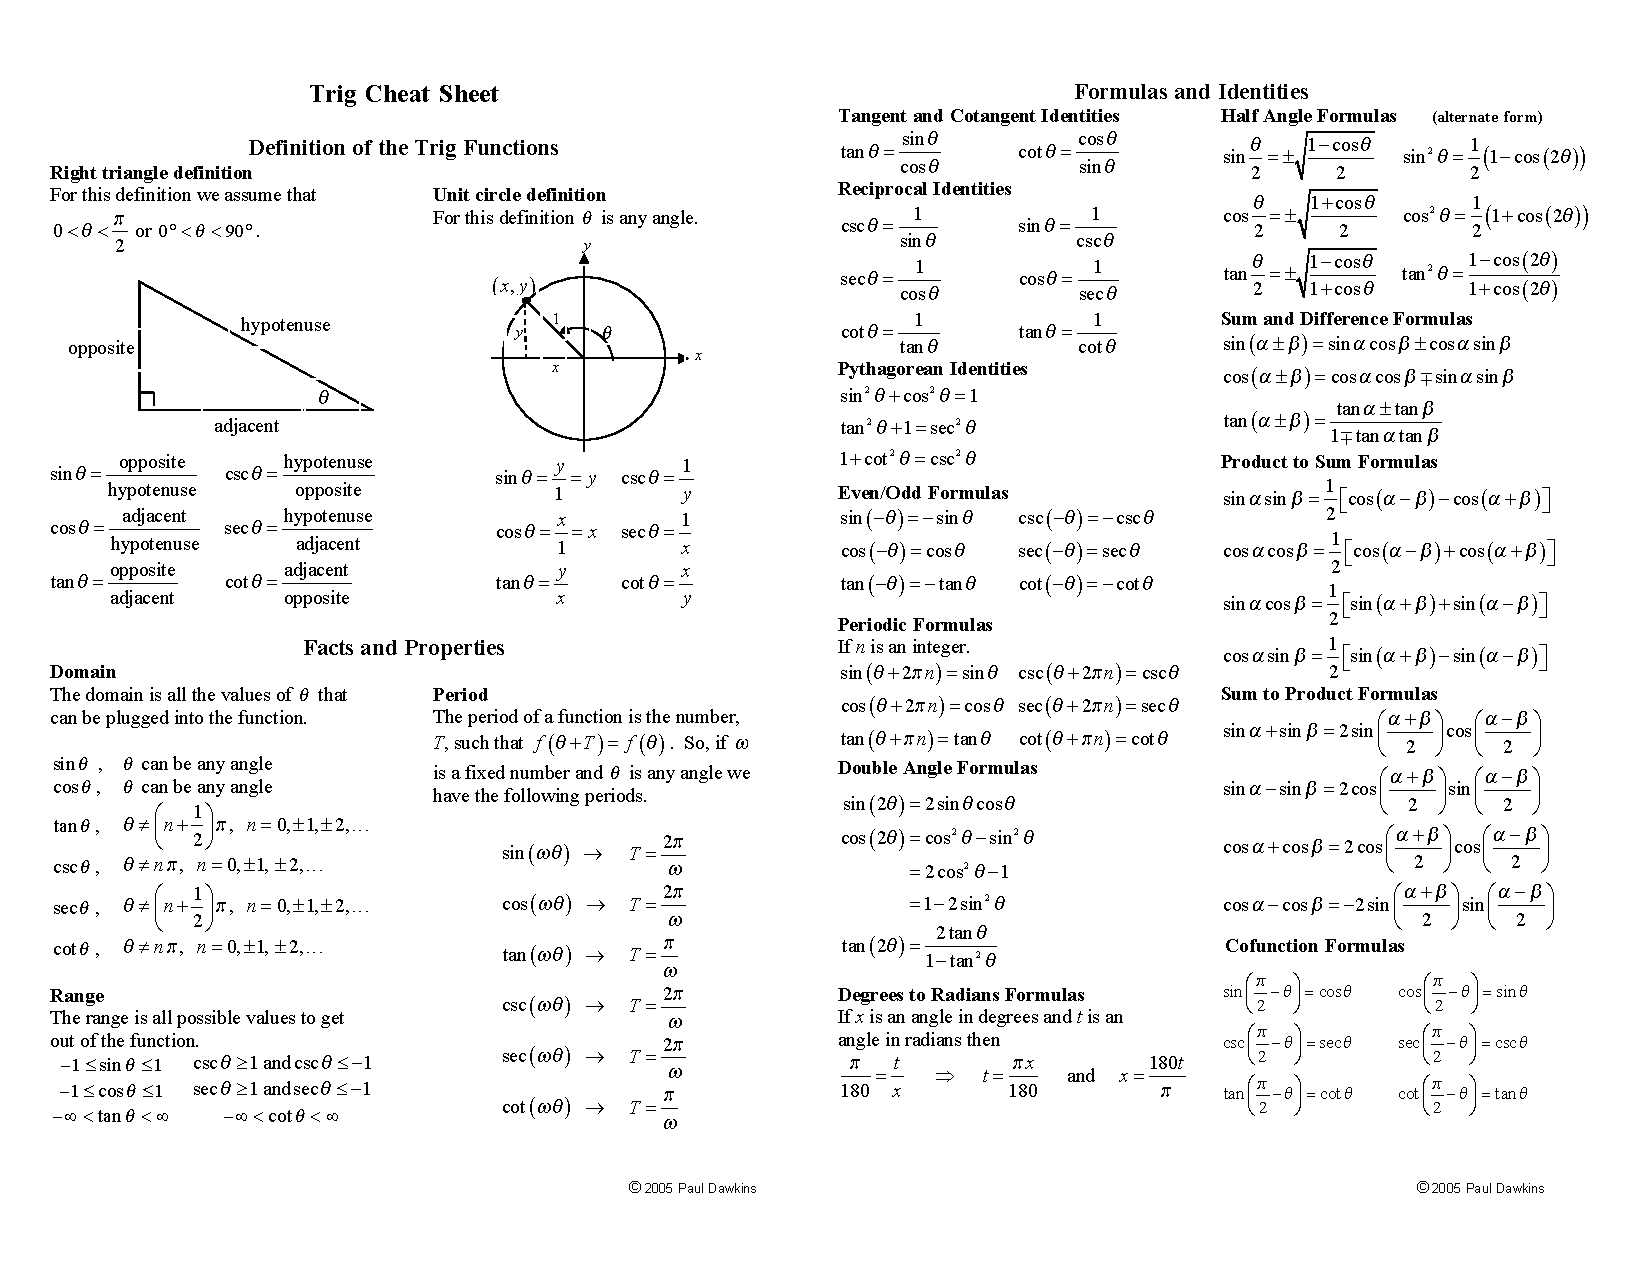
\includepdf[pages={1-},scale=1, angle=90]{Math/Trig_Cheat_Sheet_Reduced.pdf}

\end{multicols}
\end{landscape}

\end{document}

